\documentclass{article}
\usepackage{tikz}
\usetikzlibrary{arrows,positioning,shapes.geometric}

\title{%
Redes Neuronales \\
Análisis del modelo de Lotka Volterra \\*[23pt]
Trabajo Práctico 1 \\
}
\date{2020}
\author{Igor Andruskiewitsch}

\begin{document}
    \maketitle
    \pagenumbering{arabic}

\section{Introducción}

\subsection{Modelo Lotka-Volterra}

Este trabajo está orientado a comprender el {\bf Modelo de predadores y prezas de Lotka-Volterra}, descrito como el sistema de dos ecuaciones diferenciales ordinarias (ODEs):

$$ \dot{C}(t) = \alpha C(t) - \beta C(t) Z(t) $$
$$ \dot{Z}(t) = - \gamma Z(t) + \delta C(t) Z(t) $$

Donde:

\begin{itemize}
    \item {$ C(t) $ modela el número de presas de un ecosistema}
    \item {$ Z(t) $ modela el número de depredadores en el mismo ecosistema}
\end{itemize}

\subsection{Objetivos}

\begin{itemize}
    \item {Comprender las herramientas disponibles para analizar ODEs}
    \item {Utilizar estas herramientas para comprender el comportamiento del modelo de Lotka-Volterra y extraer conclusiones}
\end{itemize}

\subsection{Parámetros}

Se considerarán los siguientes valores para los parámetros:

$$ \alpha = 0.1 \qquad \beta = 0.02 \qquad \gamma = 0.3 \qquad \delta = 0.01 $$

\section{Diagrama de flujo}

Para comprender el comportamiento del modelo, debemos comenzar por entender su flujo, es decir, la tendencia de crecimiento/decrecimiento de nuestras presas/depredadores y su relación.
Podemos considerar 4 diferentes estados:

\begin{center}
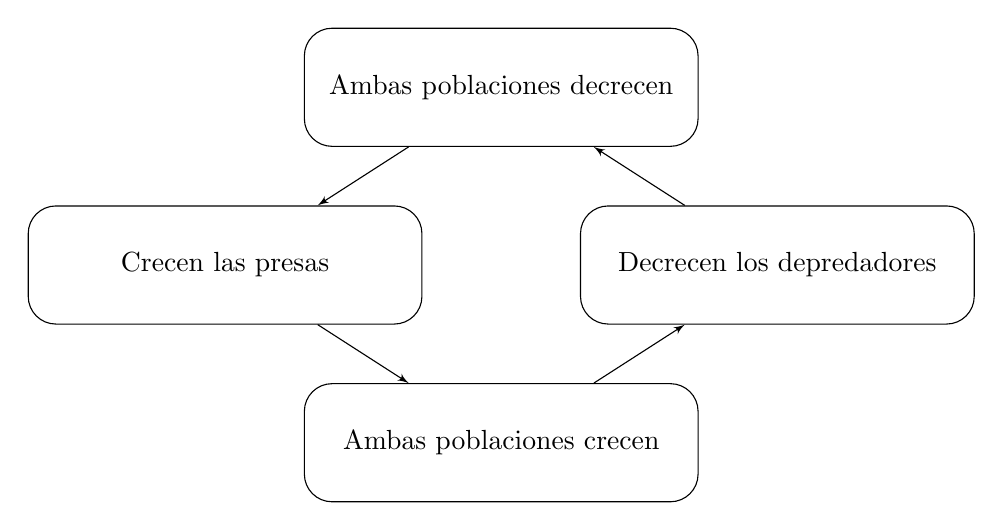
\begin{tikzpicture}[>=latex']
        \tikzset{
            block/.style= {
                draw,
                shape=rectangle,
                align=center,
                rounded corners=1em,
                minimum width=5cm,
                minimum height=1.5cm
            },
        }
        \node [block] (decrecen)
            {Ambas poblaciones decrecen};
        \node [block, below =3cm of decrecen] (crecen)
            {Ambas poblaciones crecen};
        \node [block, below left =1.5cm and =3cm of decrecen] (crecen_p)
            {Crecen las presas};
        \node [block, below right =1.5cm and =-3cm of decrecen] (crecen_d)
            {Decrecen los depredadores};
%% paths
\path[draw,->] 
    (decrecen) edge (crecen_p)
    (crecen) edge (crecen_d)
    (crecen_p) edge (crecen)
    (crecen_d) edge (decrecen)
;
\end{tikzpicture}
\end{center}

\section{Diagrama de fase}

El diagrama de fase es otra herramienta que nos permite entender la relación entre las poblaciones. Vamos a aproximar las tasas de crecimiento de ambas poblaciones utilizando el algoritmo de Runge Kutta de 4to orden, utilizando distintos puntos iniciales para observar las tendencias en la relación. A su vez, vamos a mostrar en conjunto los vectores que indican la dirección:



\end{document}
